\def\theauthor{Peter Boström, Andreas Tarandi} % TODO: stoppa in ditt namn här
\def\homeworknumber{ALS} % TODO: stoppa in vilken hemläxa det är här
\def\coursename{Fysik} % TODO: stoppan in kursnamn här
\def\course{SK1131} % TODO: stoppa in kurskod här
\def\thedate{2009-12-15}

\documentclass[a4paper,10pt]{article}
\usepackage[inner=3cm,top=3cm,outer=2cm,bottom=3cm]{geometry}
\usepackage[swedish]{babel}
%\usepackage[T1]{fontenc}
\usepackage[utf8]{inputenc}
\usepackage{graphicx}

\title{Hemläxa \homeworknumber\ - \course\ \coursename}
\date{\thedate}
\author{\theauthor}

\begin{document}
\maketitle % skapa titelsida
	\thispagestyle{empty}
\newpage % ny sida
\thispagestyle{empty}
\tableofcontents % innehållsförteckning
\newpage

% TODO: stoppa in faktiskt innehåll här.

\section{Atomspektroskopi}

\subsection{Kalibrering av mätinstrument}

Först sorterades de filter vi hade efter färg på ljus som passerade genom dem från taklampan. Dessa placerades i motsvarande fack.

För att kalibrera mätinstrumentet efter våglängd så behövde vi få ut 7 olika våglängder och vilka kanaler de svarade mot. De fyra filter vi hade svarade mot 4 av dessa kanalerna. Vi fick även spetsvärden som svarade till andra diffraktionsordningen för 3 av dessa. Dessa toppar används för att simulera värden för dubbla våglängderna av detta ljus, då apparaturen ändast känner av uppmätt densitet.

\begin{center}
\begin{tabular}[c]{|l|l|}
	\hline
	Våglängd & Kanal \\
	\hline
	404,7nm & 626 \\
	435,8nm & 686 \\
	546,1nm & 896 \\
	578,0nm & 960 \\
	\hline
	$2\lambda$ & (2:a diffr.) \\
	\hline
	809,4nm & 1931 \\
	871,6nm & 1515 \\
	1092nm & 1931 \\
	\hline
\end {tabular}
\end {center}
\vspace{10pt}

Vi fick två toppar för 578 nanometer som sammanföll till mindre toppar i kanal 975 och 960. Vi valde topp 960 efter rådfrågning då den gav ett mindre fel vid anpassning (mindre fel). Det största felet gavs då som 0.8 (nm).

\subsection{Okänd gas}

Med hjälp av funna spektrallinjer så ska vi hitta vilken gas som finns i en viss lampa. Vi skulle finna de våglängder dessa linjer svarar mot och slå upp det ämne som skickar ut dessa våglängder i en tabell.

Vi fann att ämnet som linjerna svarade bäst mot var kvicksilver. Vi fick däremot även in lite skräpljus som inte svarade mot någon av våglängderna. Självklart fick vi även dubbla våglängder för dessa linjer som svarar mot andra diffraktionsnivån.

\begin{center}
\begin{tabular}[c]{|r|r|}
	\hline
	Uppmätt frekvens (nm) & Tabellvärde (nm) \\
	\hline
	357.8 & ? \\
	367.0 & ? \\
	405.8 & ? \\
	436.0 & ? \\
	547.4 & ? \\
	$2\lambda$ & -- \\
	764.8 & -- \\
	816.6 & -- \\
	845.7 & -- \\
	914.6 & -- \\
	1097.0 & -- \\
	\hline
\end{tabular}
\end{center}

\subsection{Balmerlinjer för väte och svarande rydbergskonstanter}

Vi mätte de våglängder som emitterades från en vätelampa. Detta gav oss fem olika våglängder som svarar mot linjer $H_\alpha$ till $H_\epsilon$.

Rydbergs konstant mäts upp med ekvationen:

\begin{eqnarray*}
\frac{1}{\lambda} &=& R\left(\frac{1}{n^2_1} - \frac{1}{n^2_2}\right) \\
R &=& \lambda^{-1}\left(\frac{1}{n_1^2} - \frac{1}{n_2^2} \right)^{-1}
\end{eqnarray*}

Där $n_1 = 2$ i Balmerserien. Vilket ger:

$$ R = \lambda^{-1}\left(\frac{1}{4} - \frac{1}{n^2}\right)^{-1} $$

Mätvärden och uträkningar ger oss följande:

\begin{center}
\begin{tabular}[c]{|r||r|r||r|r||r|}
	\hline
	Linje & $\lambda (nm)$ & Rydbergs konstant & $\lambda (nm)$, tabell & Rydbergs (tabell) & Avvikelse (andel) \\
	\hline
	\hline
	$H_\alpha$ & 662.4 & $1.087*10^7$ & 656.3 & $1.097*10^7$ & $9.49*10^{-3}$ \\
	$H_\beta$ & 486.4 & $1.096*10^7$ & 486.1 & $1.097*10^7$ & $8.04*10^{-4}$ \\
	$H_\gamma$ & 436.4 & $1.091*10^7$ & 434.1 & $1.097*10^7$ & $5.64*10^{-3}$ \\
	$H_\delta$ & 413.0 & $1.090*10^7$ & 410.2 & $1.097*10^7$ & $7.09*10^{-3}$\\
	$H_\epsilon$ & 399.0 & $1.092*10^7$ & 397.0 & $1.097*10^7$ & $5.24*10^{-3}$ \\
	\hline
\end{tabular}
\end{center}

Våra experimentellt uppmätta rydbergskonstanter skiljer sig inte mer än någon procent från tabellvärdet. Standardavvikelsen ligger på $328.9$. Detta är bra.

\subsection{Elektronvoltsdiagrammet}

Våra övergångar svarar mot övergångar:

\begin{center}
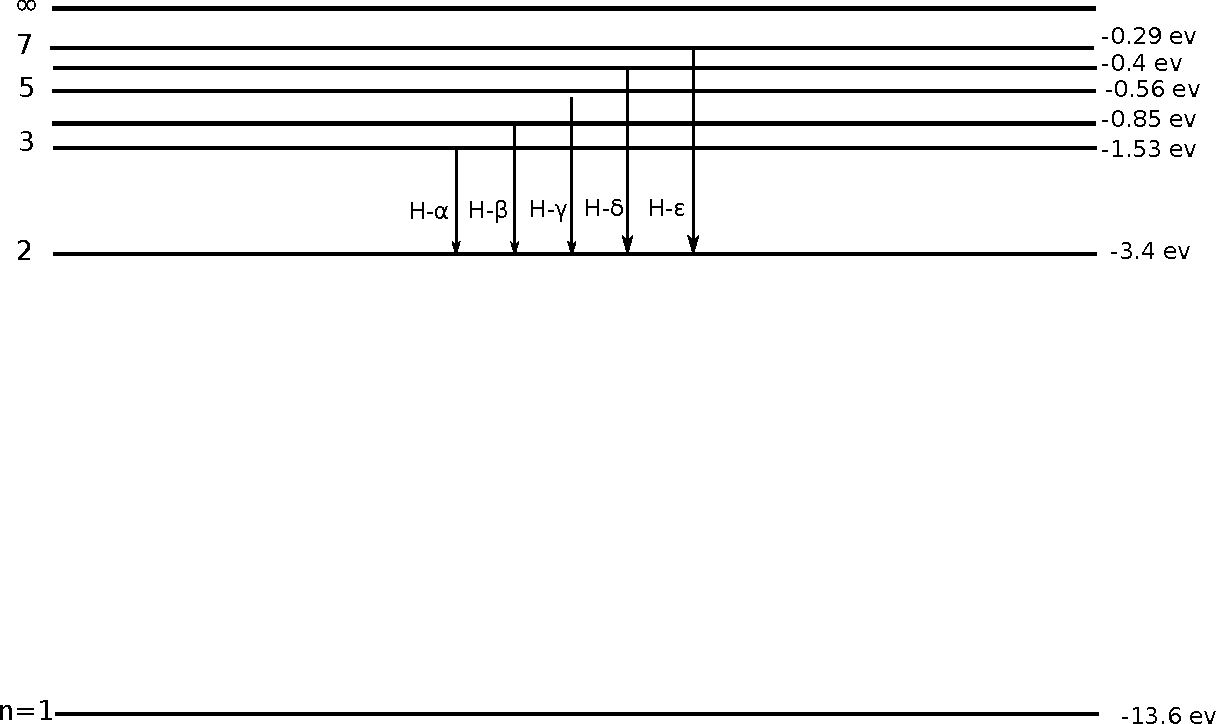
\includegraphics[width=120mm]{als-elektron}
\end{center}

\newpage

\section{Laser} % (fold)

\subsection{Mätningar av våglängder och deras vågtal}
\begin {center}
\begin {tabular}[c]{|r|r|}

	\hline
	Våglängd (topp) & Vågtal ($\sigma = cm^{-1}$)\\
	\hline
	544,2 & $ 1.84*10^4$ \\
	550,0 & $ 1.82*10^4$ \\
	556.5 * & $ 1.80*10^4$ \\
	563,1 & $ 1.78*10^4$ \\
	569.9 * & $ 1.75*10^4$ \\
	576,7 & $ 1.73*10^4$ \\
	583,5 * & $ 1.71*10^4$ \\
	590,4 & $ 1.69*10^4$ \\
	597,7 & $ 1.67*10^4$ \\
	605.3 * & $ 1.65*10^4$ \\
	612,9 & $ 1.63*10^4$ \\
	620.3 * & $ 1.61*10^4$ \\
	627,7 & $ 1.59*10^4$ \\
	635.6 * & $ 1.57*10^4$ \\
	643,4 & $ 1.55*10^4$ \\
	652,4 & $ 1.53*10^4$ \\
	661,3 & $ 1.51*10^4$ \\
	669,8 & $ 1.49*10^4$ \\
	678.0 * & $ 1.47*10^4$ \\
	686,1 & $ 1.46*10^4$ \\
	695.6 * & $ 1.44*10^4$ \\
	705,1 & $ 1.42*10^4$ \\
	714,6 & $ 1.40*10^4$ \\
	725,2 & $ 1.38*10^4$ \\
	733,6 & $ 1.36*10^4$ \\
	743,1 & $ 1.35*10^4$ \\
	753,1 & $ 1.33*10^4$ \\
	764,2 & $ 1.31*10^4$ \\
	773,2 & $ 1.29*10^4$ \\
	783,8 & $ 1.28*10^4$ \\
	\hline

\end {tabular}
\end {center}

Alla våglängder markerade med * räknades ut i efterhand där mätvärden saknades.

\newpage

\section{Vågtalsskillnader och $\omega$}

Med givna uträknade vågtal kan vi beräkna $\omega_e$ och $\omega_e\chi_e$:

$$ \sigma_v - \sigma_{v+1} = \omega_e - 2\omega_e\chi_e - 2v\omega_e\chi_e $$

Detta ger oss en linjär ekvation där $k = -2\omega_e\chi_e, x = v $ och $ m = \omega_e - 2\omega_e\chi_e $ i linjära ekvationen $y=kx+m$.

Linjär minstakvadrat-anpassning av punktskillnaden ger k = -1.3182 och m = 213.4704 och grafen:

\begin{center}
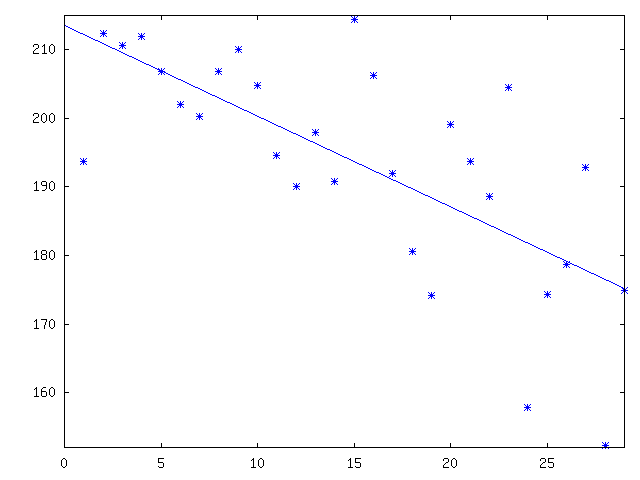
\includegraphics[width=120mm]{als-fit}
\end {center}

Från ekvationen får vi:

$$ \omega_e = 214,79 $$
$$ \omega_e\chi_e = 0.6591 $$

Tabellvärden är $214.5$ respektive $0.62$, så våra värden är rel. bra.

Energin $D_e$ ges av formeln:

$$D_e = \frac{\omega_e^2}{4\omega_e\chi_x} \approx 17500 $$

Beräkning av a:

$$ \omega_e\chi_e = \frac{ha^2}{16\pi^2c\mu} cm^{-1} $$

$$ \mu = \frac{m_I^2}{2m_I} = 1.0597*10^{-25} kg$$

$$ a = \sqrt{\frac{\omega_e\chi_e16\pi^2c\mu}{h}} \approx 2,234*10^{10} m^{-1} $$

Rotationskonstanten tabellvärdet $B_e$

$$ B_e = 0.0374 cm^{-1} $$

Tillsammans med ekvationen: 

$$ B_e = \frac{h}{8\pi^2c\mu r_e^2} $$

får vi ut att:

$$ r_e = \sqrt{\frac{h}{8*\pi^2c\mu B_e}} = 2.66*10^{-10} $$

\section{Diskussion}

Våra mätvärden för vätelampa var bra, då resultatet skiljde sig med mindre än någon procent från tabellvärden.

Våra punktskillnader vid minstakvadratanpassning var dock väldigt utspridda, men verkar ändå stämma bra överrens mot de tabellvärden som finns för $\omega_e$ och $\omega_e\chi_e$, så det var ingen större felkälla.

\end{document}
